\documentclass[11pt]{beamer}
\usepackage[utf8]{inputenc}
\usepackage[T1]{fontenc}
\usepackage{amsmath}
\usepackage{amsfonts}
\usepackage{amssymb}
\usepackage{graphicx}
\usetheme{default}

\begin{document}
	\author{Musa Baloyi}
	\title{The Elastic Stack}
	%\subtitle{Model governance for risk management}
	%\logo{}
	%\titlegraphic{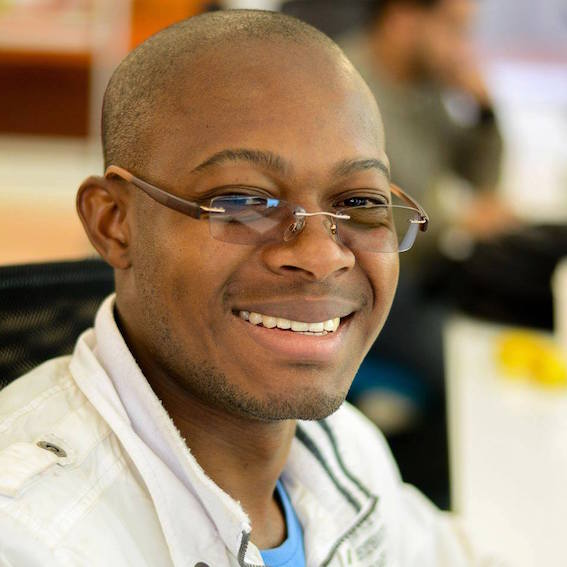
\includegraphics[width=\textwidth,height=.5\textheight]{logo}}
	%\institute{}
	%\date{}
	%\subject{}
	%\setbeamercovered{transparent}
	%\setbeamertemplate{navigation symbols}{}
	\begin{frame}[plain]
	\maketitle
\end{frame}

\begin{frame}
\frametitle{Table of contents}
\begin{itemize}
	\item The Elastic Stack
	\item Elasticsearch
	\item Logstash
	\item Kibana
	\item Beats
\end{itemize}
\end{frame}


\begin{frame}
\frametitle{The Elastic Stack}
\begin{figure}[h]
	\centering
	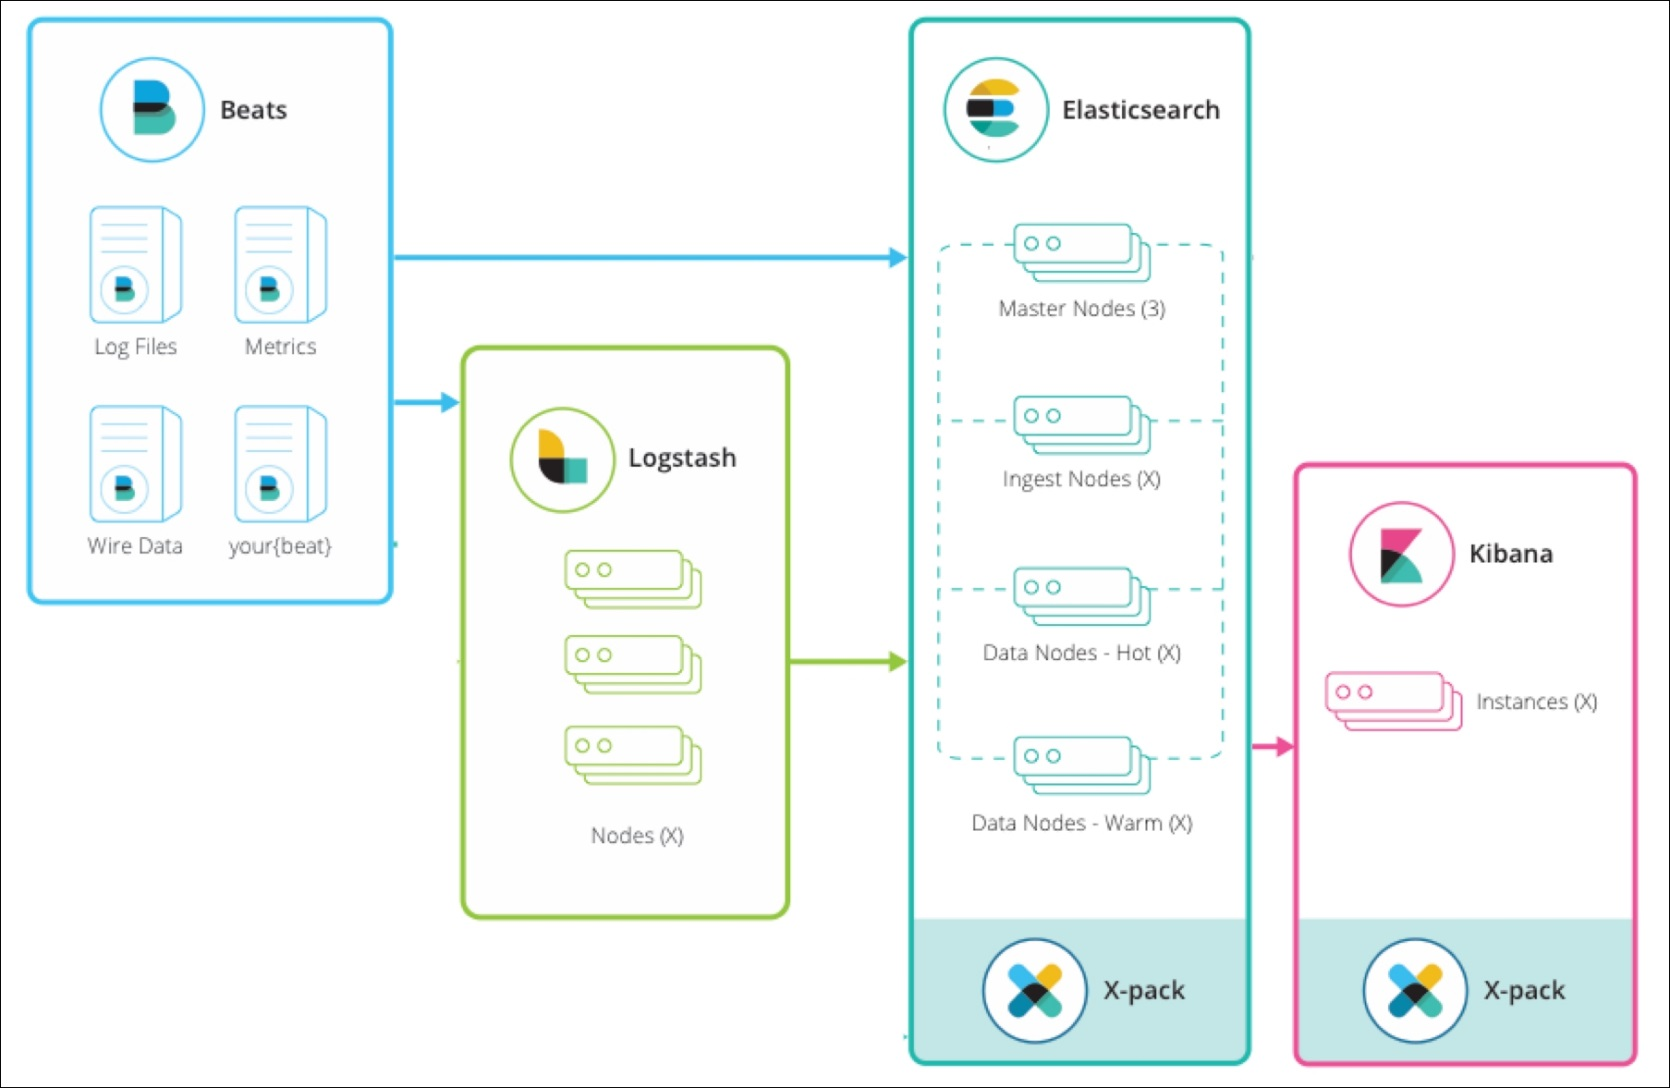
\includegraphics[scale=.5]{images/elastic_stack}
\end{figure}
\end{frame}

\begin{frame}
\frametitle{Installation guidelines}
\begin{itemize}
	\item Installing from source
	\item Using a package manager
	\item sebp/elk docker container
	\item elastic/stack-docker docker container
	\item Elastic Team SIT
	\item Elastic Team SLAM
\end{itemize}
\end{frame}

\begin{frame}
\frametitle{Elastic Stack demo}
\begin{itemize}
	\item sudo docker pull sebp/elk
	\item sudo sysctl -w vm.max\_map\_count=300000
	\item sudo docker run -p 5601:5601 -p 9200:9200 -p 5044:5044 -it --name elk sebp/elk
	\item Elasticsearch is running on http://localhost:9200
	\item Kibana is running on http://localhost:5601 
	\item Logstash started at 5044
\end{itemize}
\end{frame}

\begin{frame}
\frametitle{Elasticsearch demo}
\begin{itemize}
	\item curl -XGET 'localhost:9200/\_cat/health?v\&pretty’
	\item curl -XGET 'localhost:9200/\_cat/nodes?v\&pretty'
	\item curl -XGET 'localhost:9200/\_cat/indices?v\&pretty’
	\item Create index
\end{itemize}
\begin{figure}[h]
	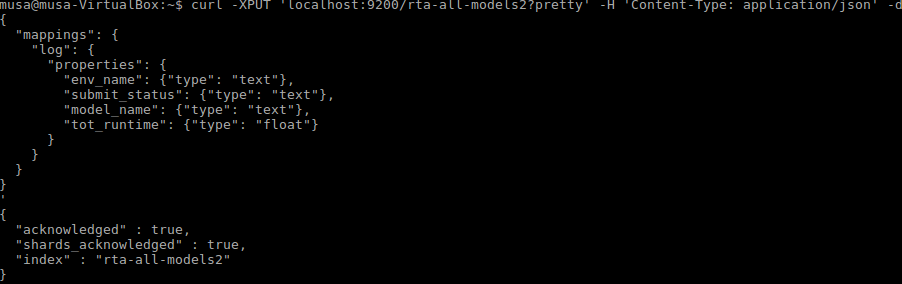
\includegraphics[scale=.4]{images/es_demo1}
\end{figure}
\end{frame}

\begin{frame}
\frametitle{Elasticsearch demo}
\begin{itemize}
	\item curl -XGET 'localhost:9200/\_cat/indices?v\&pretty’
\end{itemize}
\begin{figure}[h]
	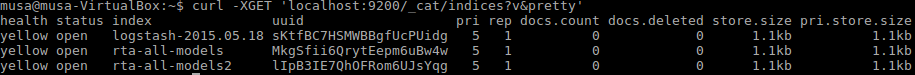
\includegraphics[scale=.4]{images/es_demo2}
\end{figure}
\begin{itemize}
	\item curl -H 'Content-Type: application/x-ndjson' -XPOST 'localhost:9200/\_bulk?pretty' --data-binary @rta\_2018-03-13T08\:37\:47.143254.json
\end{itemize}
\end{frame}

\begin{frame}
\frametitle{Elasticsearch clients}
\begin{figure}[h]
	
\includegraphics[scale=.5]{images/es_clients}
\end{figure}
\end{frame}

\begin{frame}
\frametitle{Kibana demo}
\begin{itemize}
	\item Access Kibana to see created indices and data
\end{itemize}
\begin{figure}[h]
	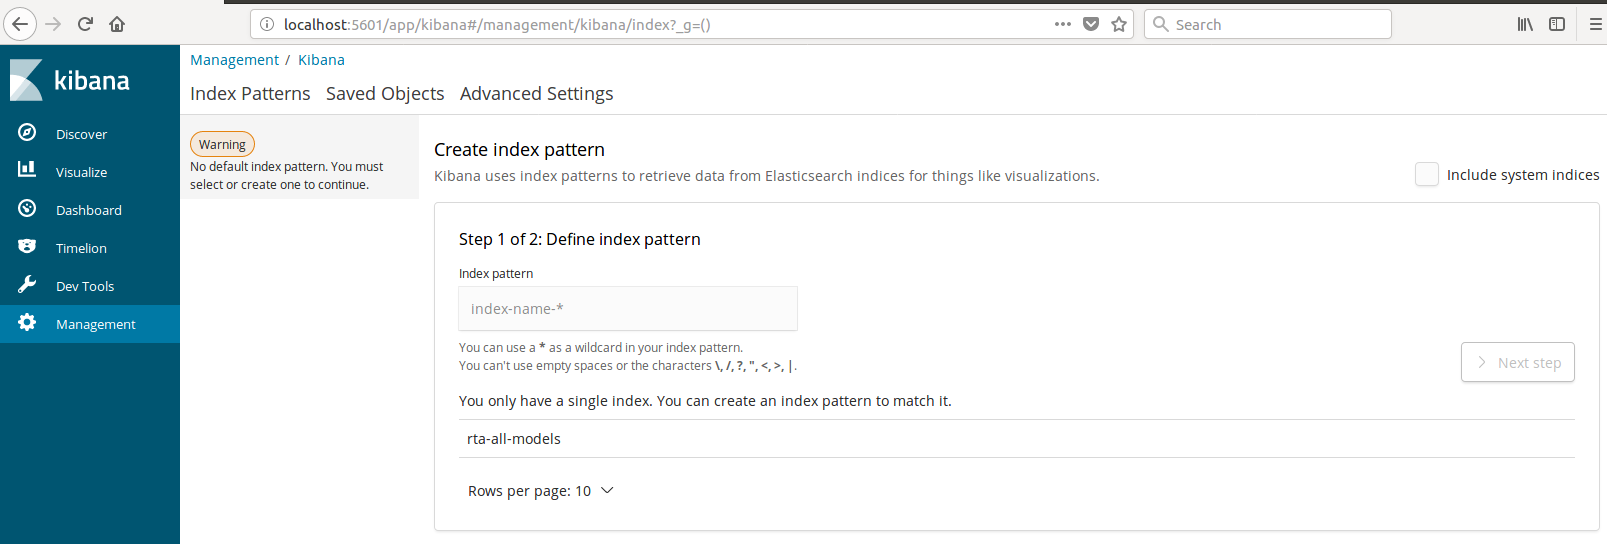
\includegraphics[scale=.25]{images/kibana1}
\end{figure}
\end{frame}

\begin{frame}
\frametitle{Kibana demo}
\begin{itemize}
	\item Create index pattern in Kibana
\end{itemize}
\begin{figure}[h]
	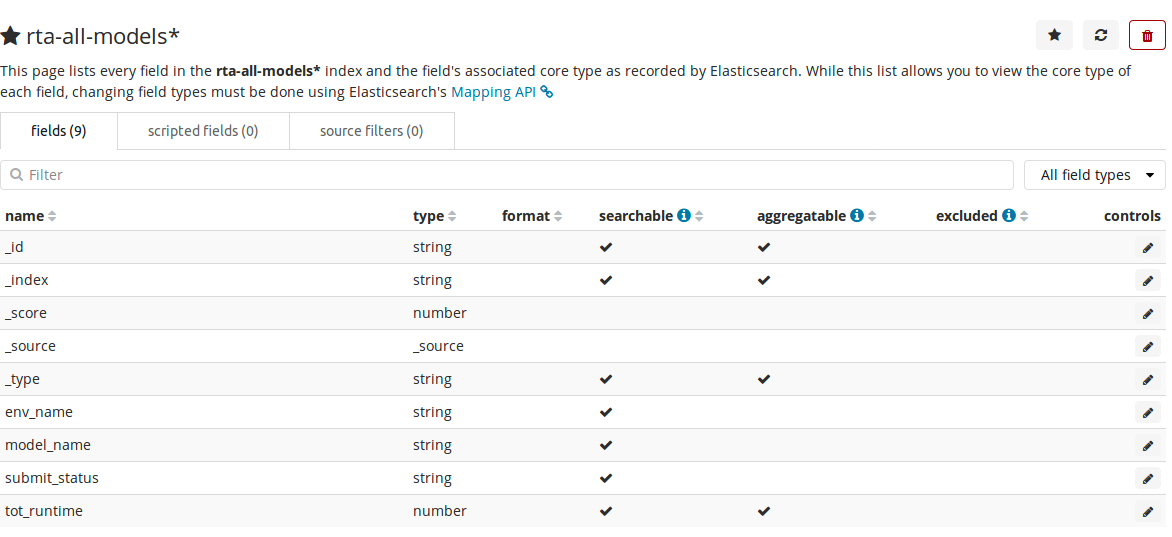
\includegraphics[scale=.3]{images/kibana2}
\end{figure}
\end{frame}

\begin{frame}
\frametitle{Kibana Console}
\begin{itemize}
	\item Alternative to CURL
\end{itemize}
\begin{figure}[h]
	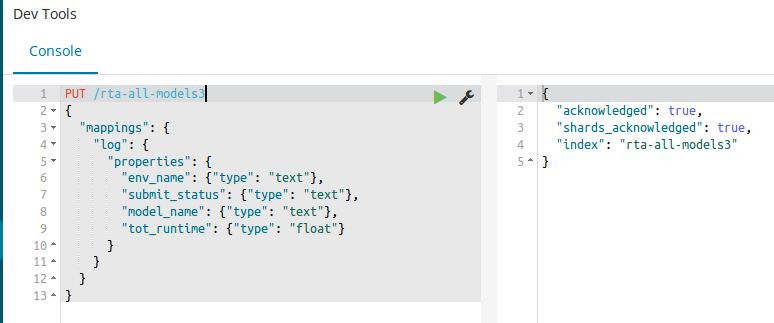
\includegraphics[scale=.5]{images/kibana3}
\end{figure}
\end{frame}

\begin{frame}
\frametitle{Elasticsearch for Hadoop}
\begin{figure}[h]
	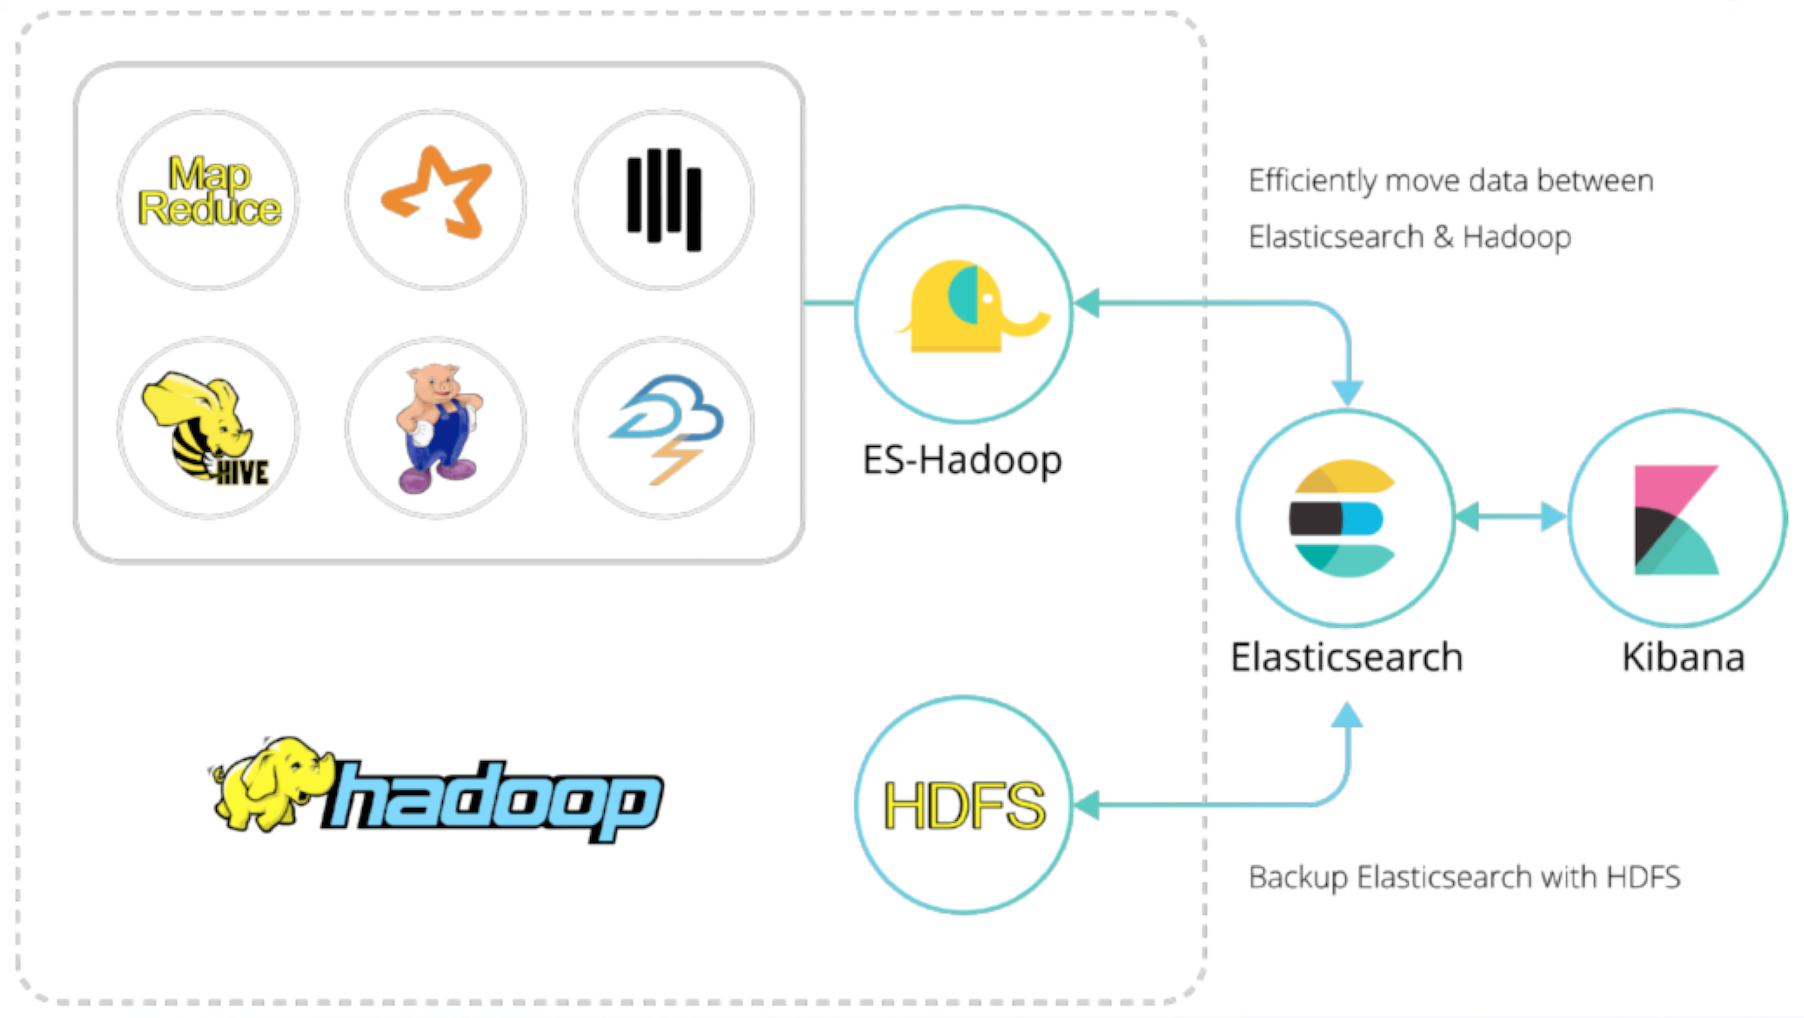
\includegraphics[scale=.3]{images/es_hdp}
\end{figure}
\end{frame}

\begin{frame}
\frametitle{Architectural overview}
\begin{figure}[h]
	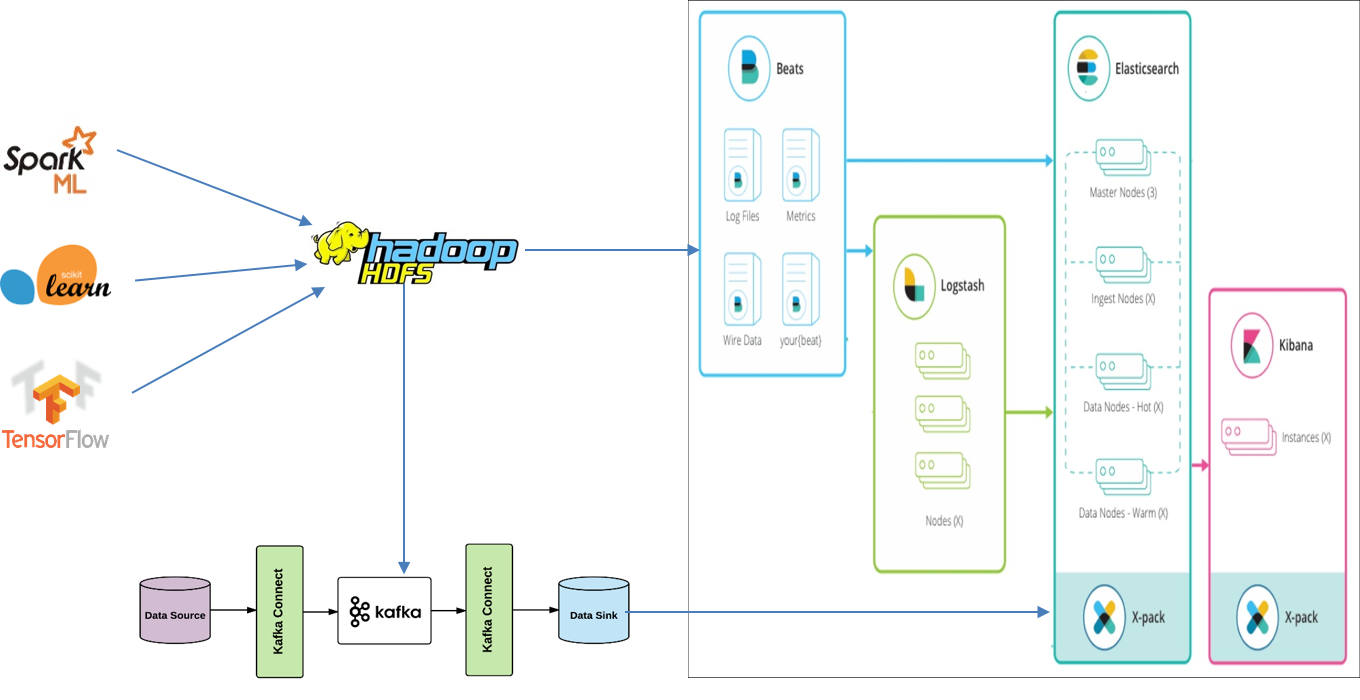
\includegraphics[scale=.3]{images/arch1}
\end{figure}
\end{frame}

\begin{frame}
\frametitle{Architectural overview}
\begin{figure}[h]
	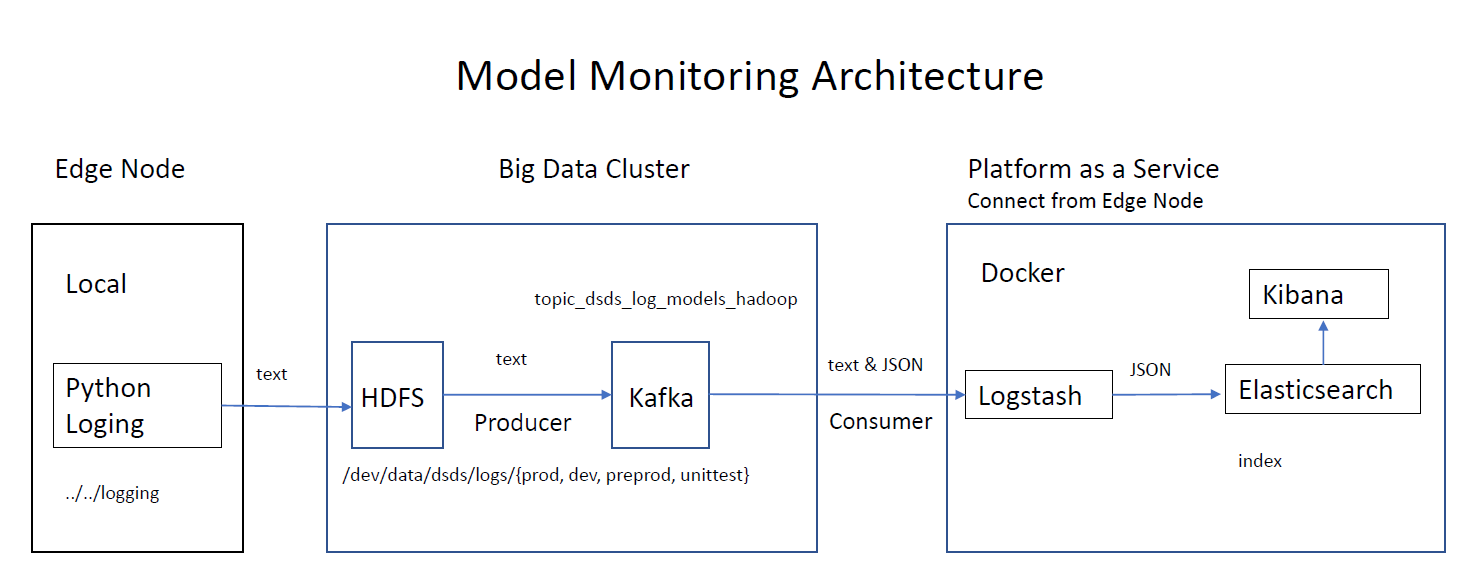
\includegraphics[scale=.3]{images/arch2}
\end{figure}
\end{frame}

\begin{frame}
\frametitle{Kafka}
\begin{itemize}
	\item Kafka is generally used for building real-time streaming 
	\begin{itemize}
		\item data pipelines that reliably get data between systems or applications
		\item applications that transform or react to the streams of data
	\end{itemize}
	\item Kafka is run as a cluster on one or more servers that can span multiple datacenters.
	\item The Kafka cluster stores streams of records in categories called topics.
	\item Each record consists of a key, a value, and a timestamp.
\end{itemize}
\end{frame}

\begin{frame}
\frametitle{Kafka installation}
\begin{itemize}
	\item Download the binary: kafka\_2.12-1.0.1.tgz 
	\item 7z x  kafka\_2.12-1.0.1.tgz \&\& 7z x  kafka\_2.12-1.0.1.tar
	\item sudo mv kafka\_2.12-1.0.1 /opt/Kafka
\end{itemize}
\end{frame}

\begin{frame}
\frametitle{Kafka demo}
\begin{itemize}
	\item cd /opt/Kafka/ kafka\_2.12-1.0.1
	\item sudo bin/kafka-server-start.sh config/server.properties
	\item bin/kafka-console-consumer.sh --bootstrap-server localhost:9092 --topic testing --from-beginning
	\item bin/kafka-topics.sh --create --zookeeper localhost:2181 --replication-factor 1 --partitions 1 --topic testing
	\item bin/kafka-topics.sh --list --zookeeper localhost:2181
	\item Configure Kafka producer connect-file-source.properties
	\item Configure Kafka consumer connect-file-sink.properties
	\item bin/connect-standalone.sh config/connect-standalone.properties config/connect-file-source.properties config/connect-file-sink.properties
\end{itemize}
\end{frame}

\begin{frame}
\frametitle{Beats}
\begin{itemize}
	\item Seamlessly integrates with the Elastic Stack. Kafka requires a separate install.
	\item One way, Kafka is bidirectional 
	\item Extensible
	\item Shippers: Filebeat, Metricbeat, Packetbeat, Winlogbeat, Auditbeat, Heartbeat.
	\item Filebeat configuration
\end{itemize}
\end{frame}

\begin{frame}
\frametitle{Beats demo: Heartbeat}
\begin{itemize}
	\item elastic/stack-docker
\end{itemize}
\end{frame}

\begin{frame}
\frametitle{Logstash.conf}
\begin{figure}[h]
	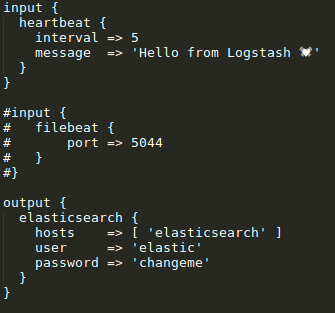
\includegraphics[scale=1]{images/logstash1}
\end{figure}
\end{frame}

\begin{frame}
\frametitle{Logstash}
\begin{itemize}
	\item grok – better pattern matching
	\item https://www.elastic.co/guide/en/logstash/current/plugins-filters-grok.html
\end{itemize}
\begin{figure}[h]
	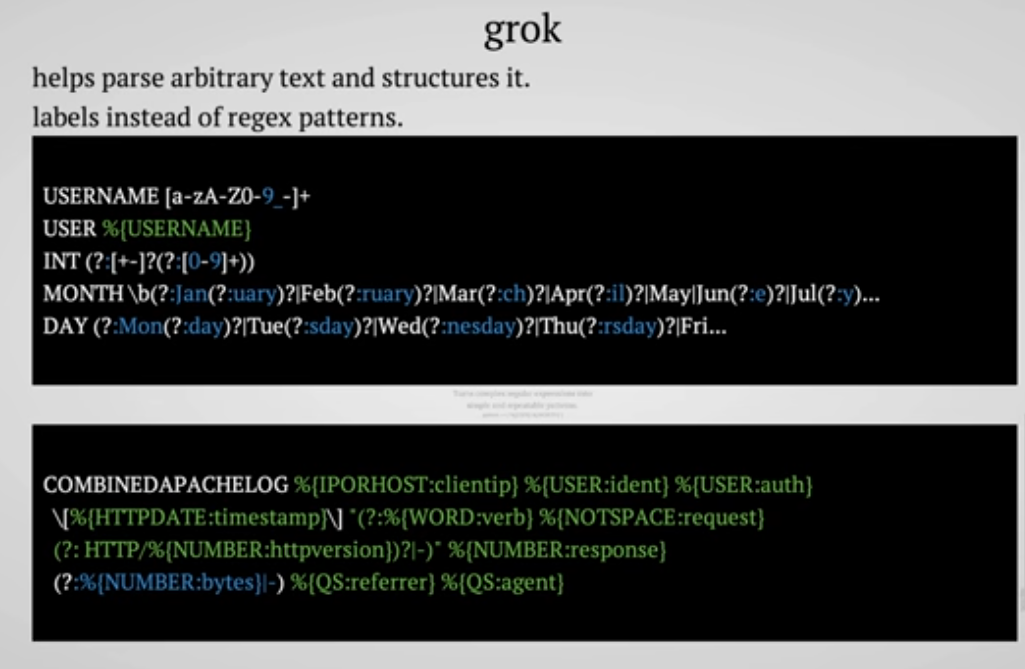
\includegraphics[scale=.3]{images/grok1}
\end{figure}
\end{frame}


\begin{frame}
\frametitle{References}
\begin{enumerate}
	\item Building Intelligent Systems: A Guide to Machine Learning Engineering. [Geoff Hulten] (Apress, 2018)
	\item Trends in AI, Data Science, and Big Data. [Ben Lorica] (2017)
	\item Building Evolutionary Architectures. [Rebecca Parsons; Patrick Kua; Neal Ford] (O'Reilly Media, 2017)
	\item 5 things you should be monitoring. [Brian Brazil] (2018)
	\item The Logstash Book. [James Turnbull] (Turnbull Press, 2013)
	\item Beyond the Twelve-Factor App. [Kevin Hoffman] (O'Reilly Media, 2016)
	\item Logs and real-time stream processing. [Jay Kreps] (2016)
	\item I Heart Logs: Apache Kafka and Real-time Data Integration. [Jay Kreps] (2015)
	\item The log: The lifeblood of your data pipeline. [Kiyoto Tamura] (2015)
	\item Understanding the ELK stack. [Brian Anderson; Rafał Kuć] (2016)
\end{enumerate}
\end{frame}

\end{document}